\begin{ex}
 As 23 ex-alunas de uma turma que completou o ensino médio há 10 anos se encontraram em uma reunião comemorativa. Várias delas haviam se casado e tido filhos. A distribuição das mulheres, de acordo com a quantidade de filhos é mostrada no gráfico abaixo:
\begin{center}
  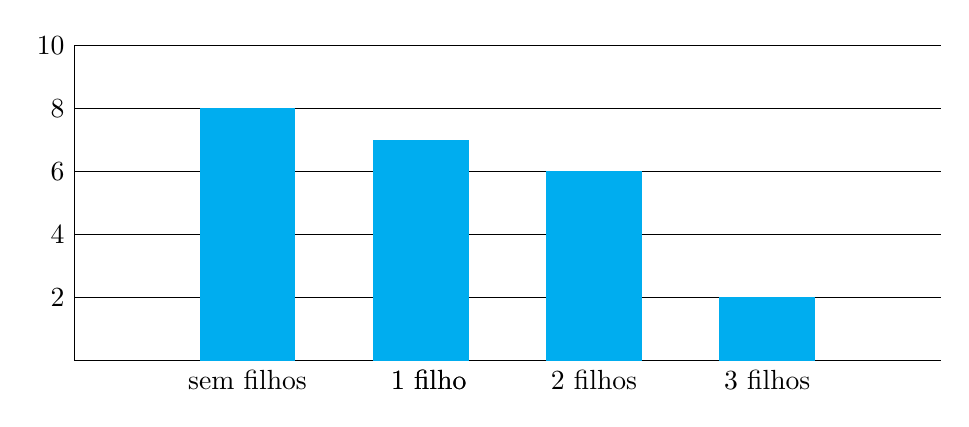
\begin{tikzpicture}
   \draw (1,0)--(12,0);\draw (1,0)--(1,4);  \draw (1,0.8)--(12,0.8); \draw (1,1.6)--(12,1.6); \draw(1,2.4)--(12,2.4);
   \draw(1,3.2)--(12,3.2); \draw (1,4)--(12,4);
   \draw[fill=cyan,draw=cyan](2.6,0)rectangle(3.8,3.2); \draw [fill=cyan,draw=cyan] (4.8,0)rectangle(6,2.8);
   \draw [fill=cyan,draw=cyan] (7,0)rectangle(8.2,2.4);\draw [fill=cyan,draw=cyan] (9.2,0)rectangle(10.4,.8);
   \node at (3.2,0)[below] {sem filhos}; \node at (5.5,0) [below] {1 filho}; \node at (5.5,0) [below] {1 filho}; \node at (7.6,0) [below] {2 filhos}; \node at (9.8,0) [below] {3 filhos};
   \node at (1,.8) [left] {2};\node at (1,1.6) [left] {4};\node at (1,2.4) [left] {6};\node at (1,3.2) [left] {8};\node at (1,4) [left] {10};
  \end{tikzpicture}
\end{center}
Um prêmio foi sorteado entre todos os filhos dessas ex-alunas. A probabilidade de que a criança premiada tenha sido um(a) filho(a) único(a), é:
   \begin{enumerate}[(a)]
   \item $\frac{1}{3}$
   \item $\frac{1}{4}$
   \item $\frac{7}{15}$
   \item $\frac{7}{23}$
   \item $\frac{7}{25}$
   \end{enumerate}
    \begin{sol}
     resposta: e \\
     número de filhos: $7+6\cdot2+2\cdot3=25 \Longrightarrow p =\frac{7}{25}$
    \end{sol}
\end{ex}